\title{Chum Populations}

\documentclass[12pt, one column]{article}
\usepackage{graphicx}
\usepackage{float}
\usepackage{enumitem}
\usepackage{lineno}
\usepackage{natbib}

\usepackage{booktabs}
\usepackage{pdflscape}
%\usepackage{fontspec}
%\setmainfont{Georgia}
%\setsansfont{Trebuchet MS}
%\setmonofont{Inconsolata}


\linenumbers
\begin{document}
% \bibliographystyle{}

\listoffigures 

\listoftables

\pagebreak
\section*{Figures}
\subsection*{Map of sampling locations including run timing}
\begin{figure}[H]
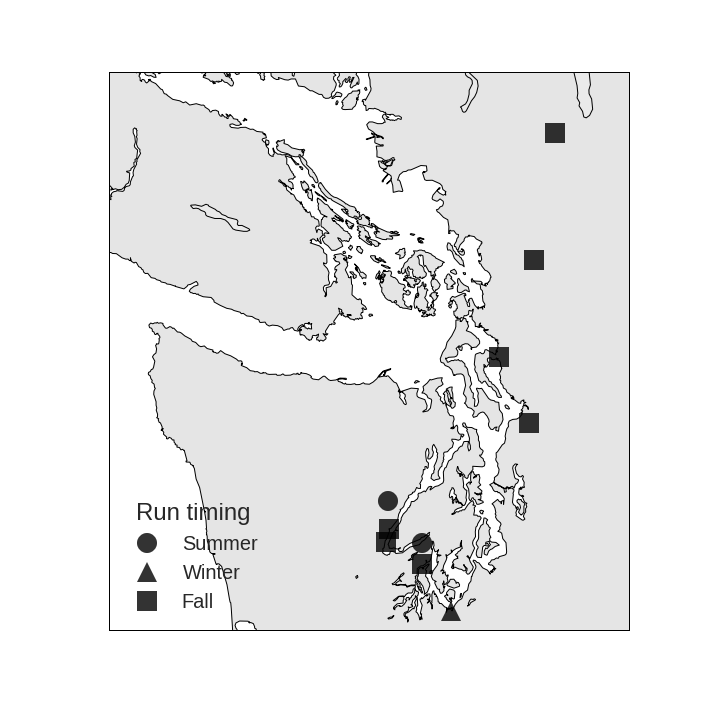
\includegraphics[scale=.6]{figures/collection_map.png}
\caption[Collection locations]{Collection locations and runtiming of chum salmon sampled near Puget Sound.}
\end{figure}

\subsection*{Linkage map}
\begin{figure}[H]
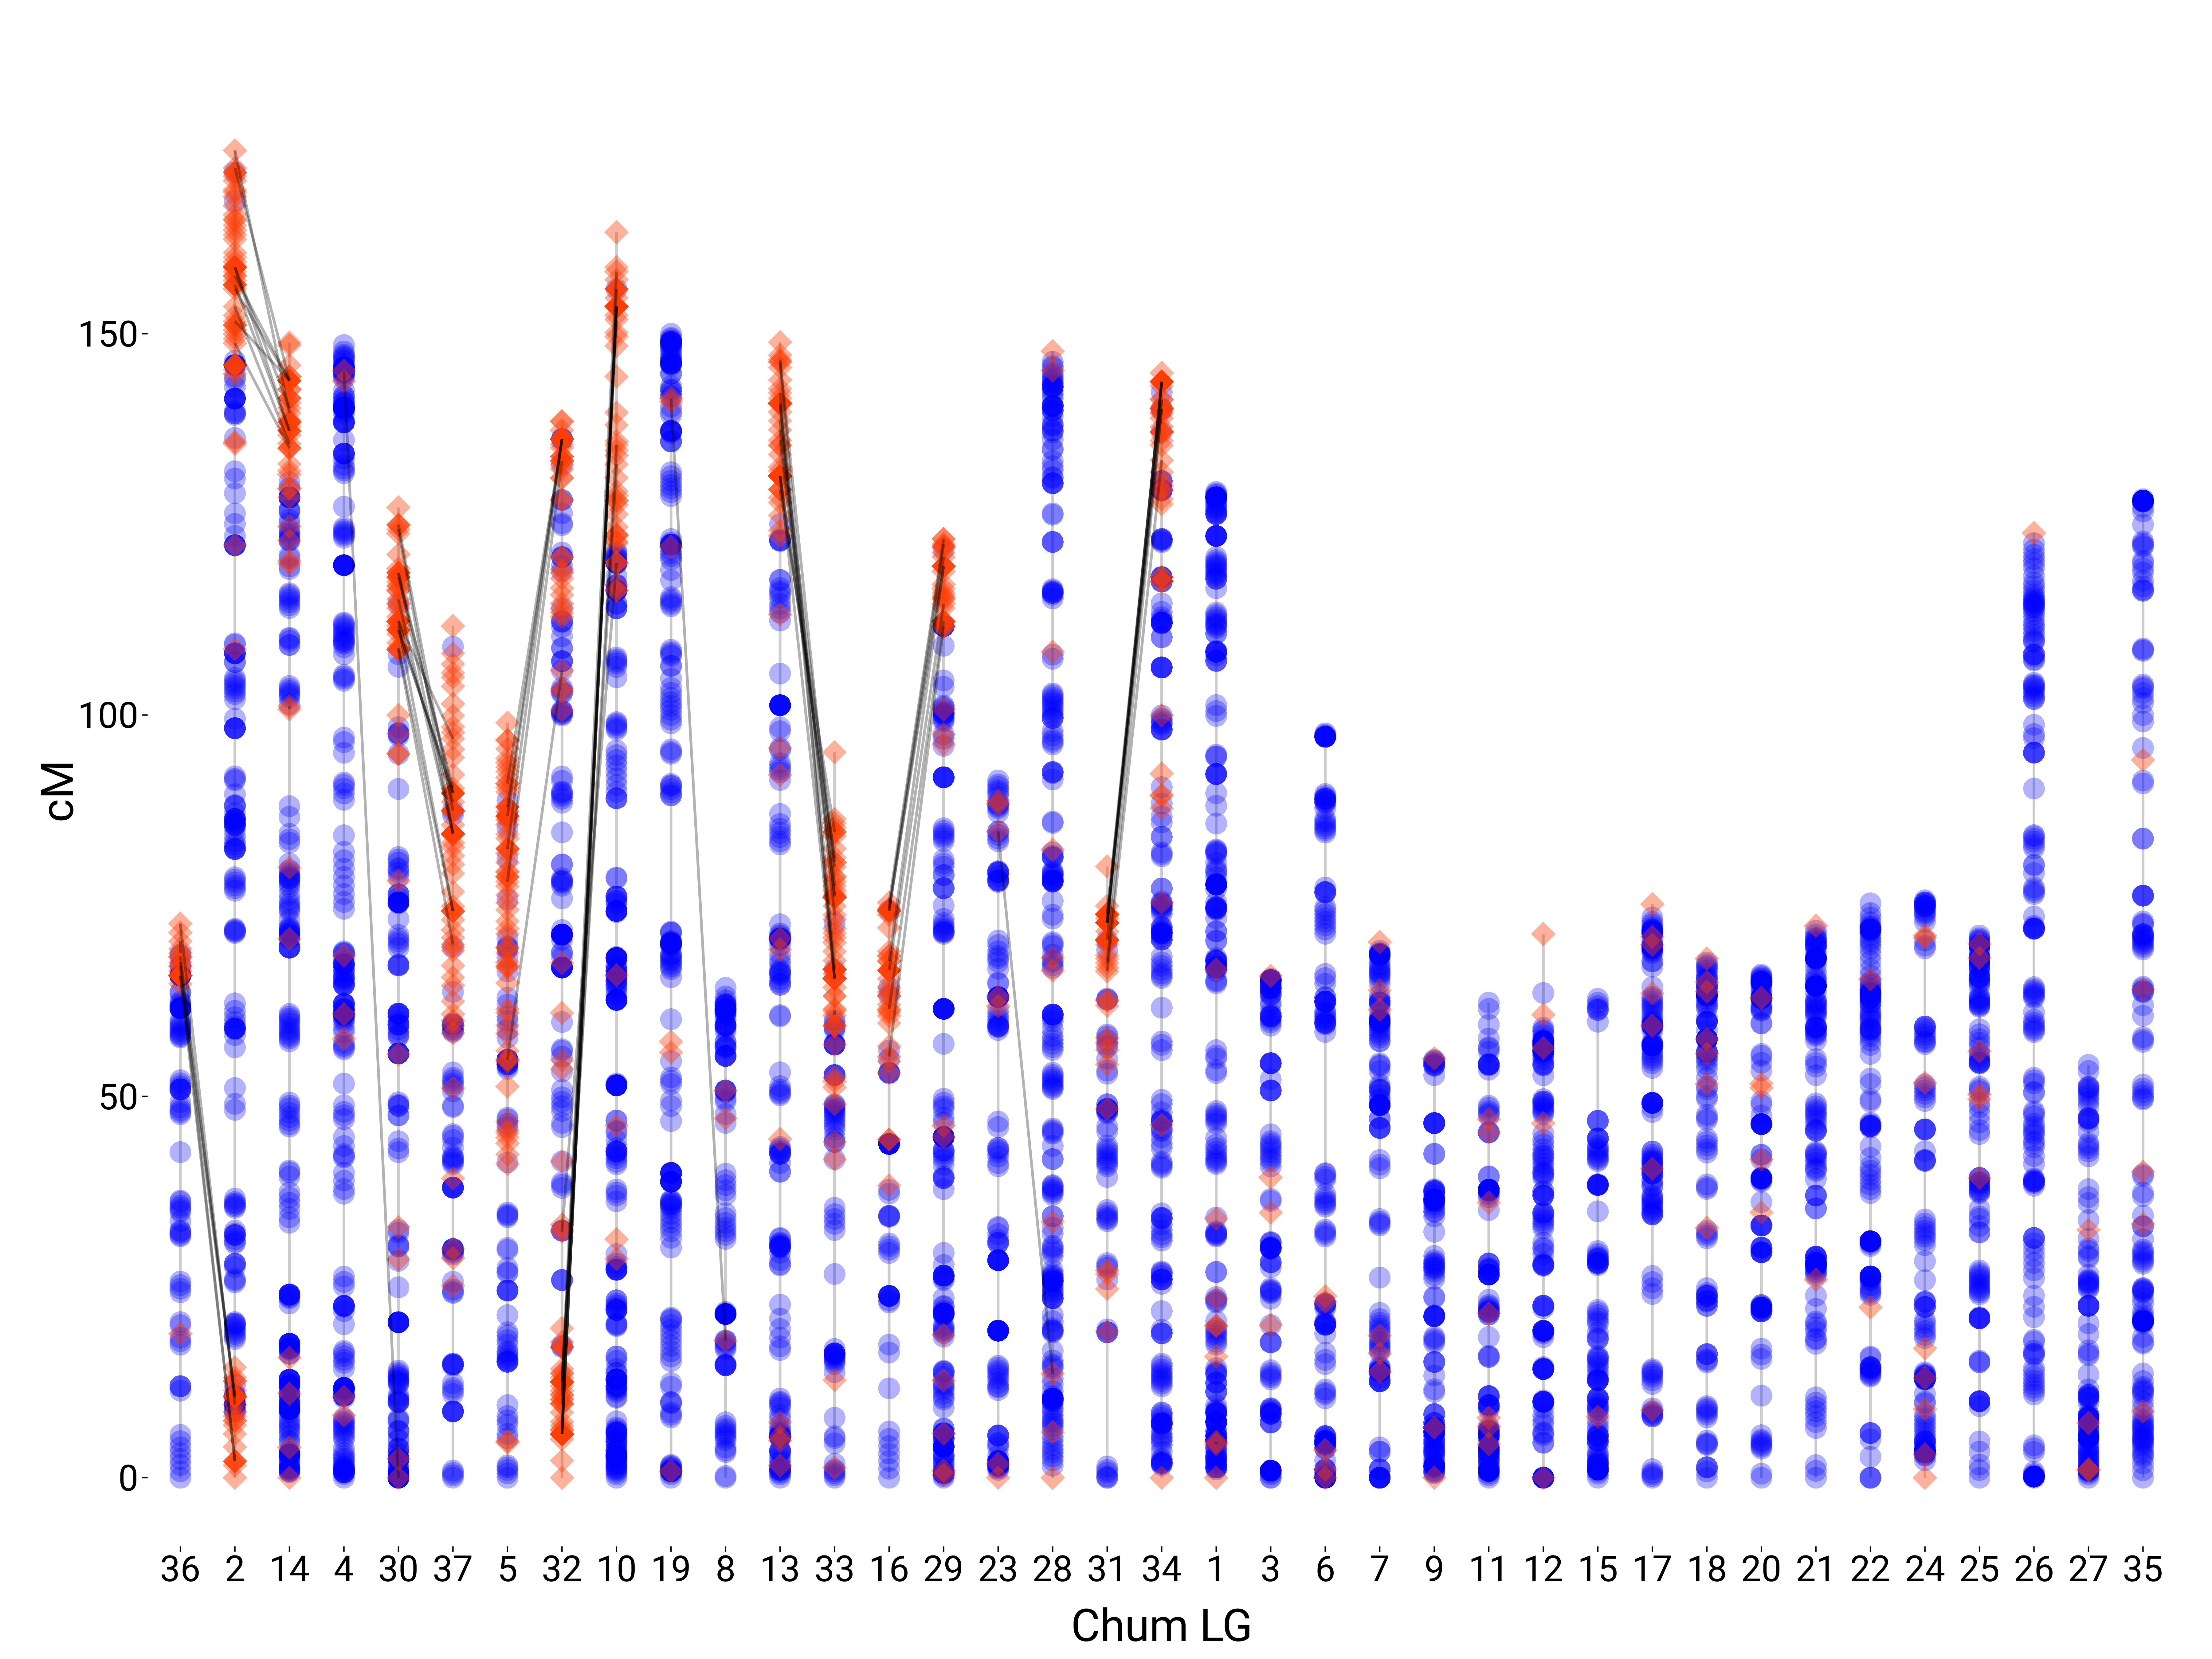
\includegraphics[scale=.26]{figures/chum_map.png}
\caption[Linkage map of chum salmon]{37 linkage groups, likely corresponding to the 37 chromosomes in the chum salmon karyotype. Paralogous loci are shown as red diamonds, non-paralogs are blue circles. Black lines connect confounded catalog entries that have been resolved into two paralogous loci. The 16 distal concentrations of paralogs form 8 pairs of homeologous chromosomes. Notice LGs 2 and 32 have distinct ancestral relationships on each end.}
\end{figure}


\subsection*{Ascertainment bias}
\begin{figure}[H]
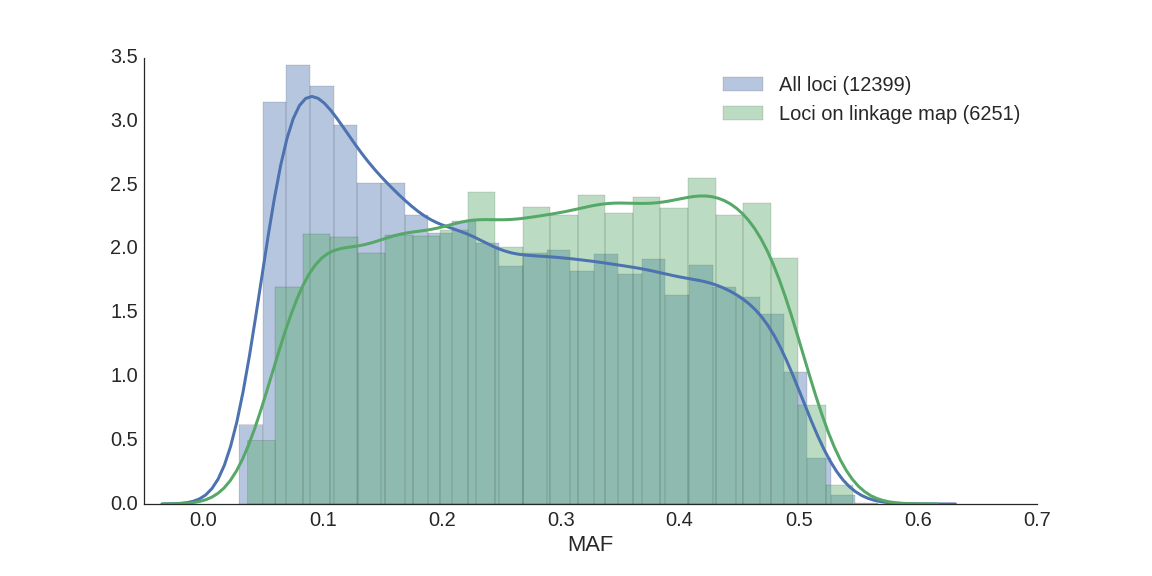
\includegraphics[scale=.5]{figures/supplemental/ascertainment.png}
\caption[MAF Histogram showing ascertainment bias]{Folded minor allele frequency (MAF) for all loci (grey) and the subset of loci placed on the linkage map (black outline). The rightward shift in the MAF distribution shows the effect of ascertainment bias.  Notice the y-axis is density-scaled to accommodate differing number of loci in each set.}
\end{figure}

\subsection*{Population structure}
\begin{figure}[H]
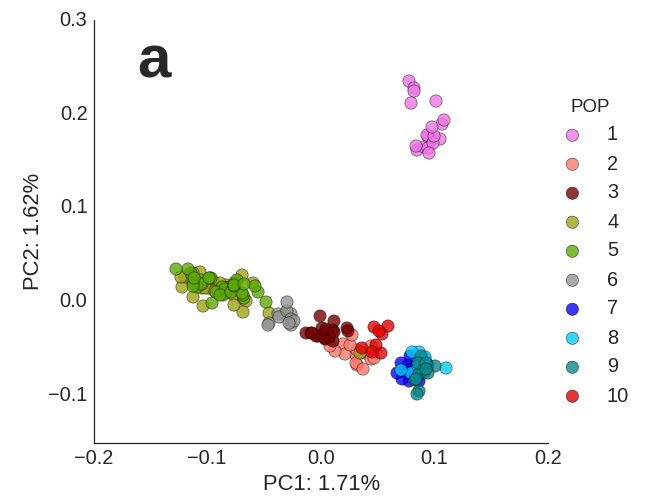
\includegraphics[scale=.35]{figures/poster_3a.png}
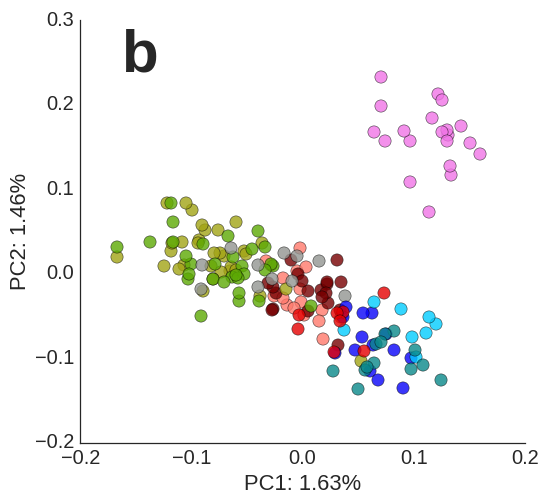
\includegraphics[scale=.35]{figures/poster_3b.png}
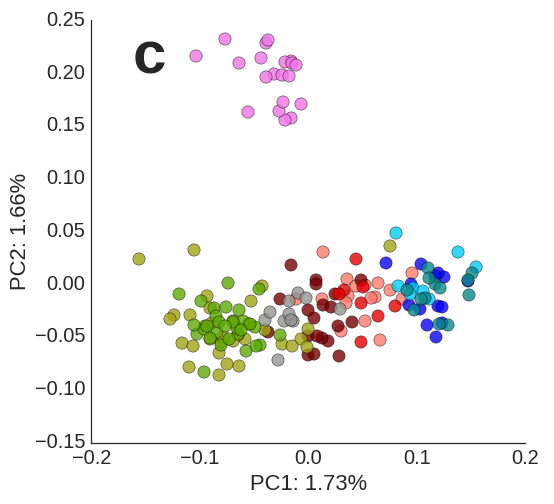
\includegraphics[scale=.35]{figures/poster_3c.png}
\caption[Individual-based PCAs showing population structure]{Population structure - Individual-based PCA from ten populations (colors) of chum salmon from Puget Sound.  Population structure obtained from paralogs (a) is similar to that obtained by non-paralogs (b), especially after down-sampling to match the number of loci (c).}
\end{figure}

\begin{landscape}
\subsection*{Manhattan plot}
\begin{figure}[H]
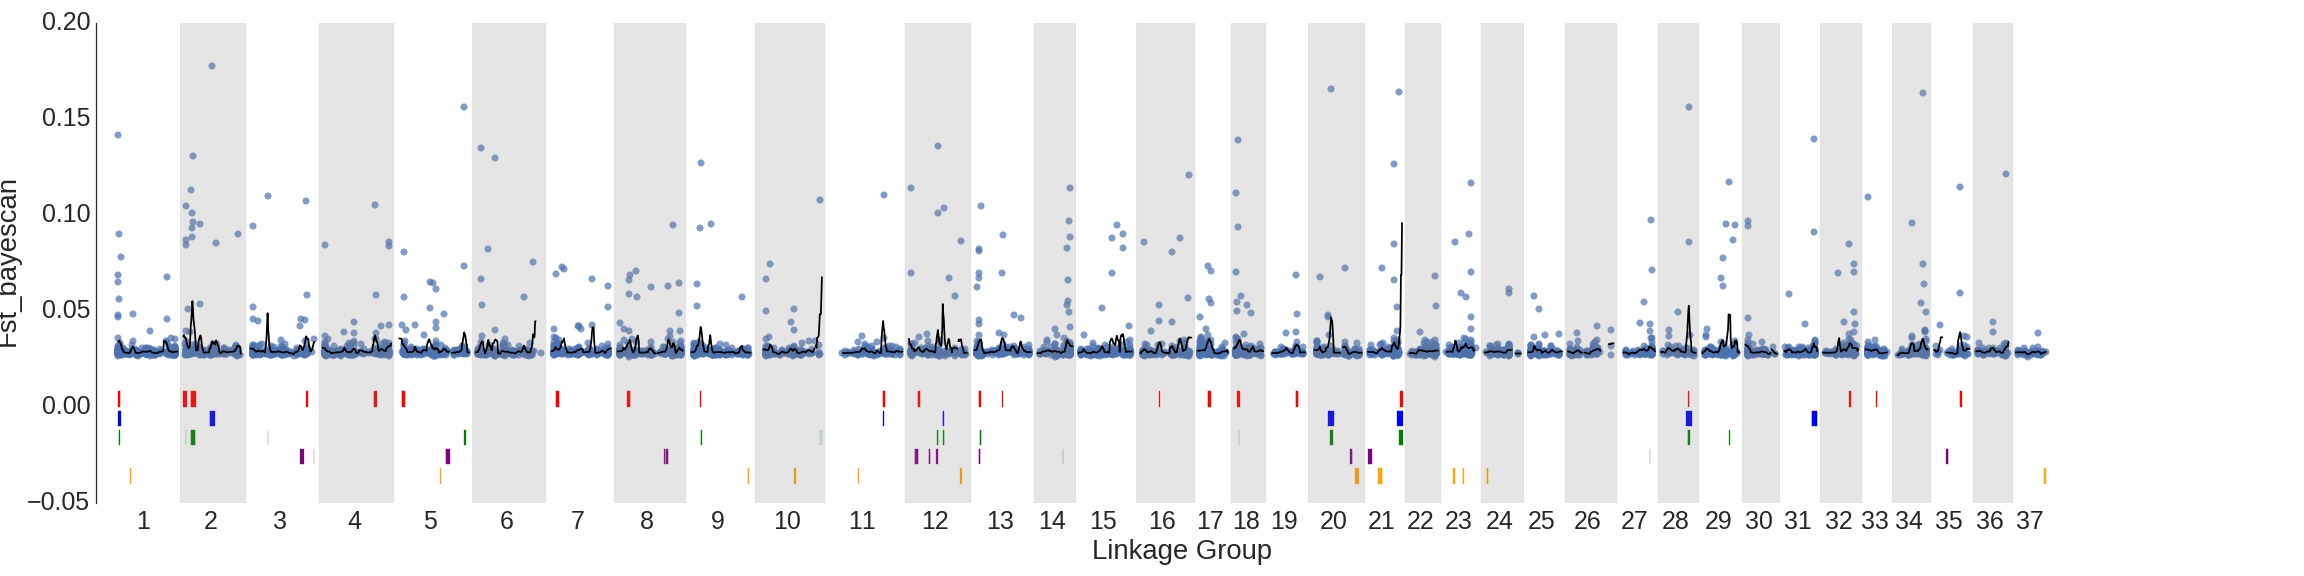
\includegraphics[scale=.25]{figures/Bayescan_Fst_and_bootstrap.png}
\caption[Manhattan plot]{Manhattan plot of differentiation across the 37 linkage groups of chum salmon.  Points are Bayescan Fst values for single loci. Population genetic statistics were calculated at each cM position by calculating an inverse distance-weighted average value from loci within a 5cM wide window centered on each position.  Black outlines show loci selected as life history outliers in Bayescan. Black Lower shaded regions show genomic regions in the upper 99\%, as determined by bootstrap permutation. Color codes for shaded regions: Red: LFMM qvalue, Blue: Bayescan qvalue, Green: Bayescan Fst, Purple: Weir Fst.}
\end{figure}
\end{landscape}
\section*{Tables}

\subsection*{Sequencing and genotyping}

\begin{table}[H]
\caption{\label{tab:table-name}Sample sizes. usable sequences, and genotyping rates}

\begin{tabular}{lrrrrr}
\toprule
{} & {} & \multicolumn{2}{c}{Aligned sequences} & \multicolumn{2}{c}{Genotyping rate}\\
Collection &  n   &            mean &        std &              mean &       std \\
\midrule
Hamma Hamma            &  20 &         1,419,541 & 1,427,760 &            0.87 &       0.08 \\
Lilliwaup Creek        &  20 &         2,760,125 &   999,141 &            0.98 &       0.01 \\
Nisqually Kalama Creek &  17 &         2,270,022 & 1,432,866 &            0.96 &       0.03 \\
Sherwood River Fall    &  32 &         3,235,188 &   966,091 &            0.96 &       0.04 \\
Sherwood River Summer  &  31 &         2,504,974 & 1,183,089 &            0.91 &       0.07 \\
Skookum Creek          &  11 &         1,644,932 &   637,844 &            0.95 &       0.09 \\
Snohomish River        &  14 &         1,135,085 &   495,888 &            0.94 &       0.07 \\
Squakum Creek          &   8 &           999,084 &   650,927 &            0.86 &       0.08 \\
Stillaguamish River    &  13 &           710,538 &   269,873 &            0.91 &       0.06 \\
Hoodsport Hatchery*    &   8 &           509,422 &   148,391 &            0.85 &       0.08 \\
\bottomrule
\multicolumn{6}{l}{*paired-end sequencing.}
\end{tabular}

\end {table}

\subsection*{Genetic diversity} 

\begin{table}[H]
%\caption{\label{tab:table-name}Genetic diversity}
\caption{Genetic diversity} 
\begin{tabular}{lrr}
\toprule
{} & Heterozygosity &     Ne \\
\midrule
Hamma Hamma            &           0.30 &    339 \\
Lilliwaup Creek        &           0.34 &  5,959 \\
Nisqually Kalama Creek &           0.32 &    161 \\
Sherwood River Fall    &           0.33 &    319 \\
Sherwood River Summer  &           0.31 &    145 \\
Skookum Creek          &           0.33 &  1,788 \\
Snohomish River        &           0.32 &  2,122 \\
Squakum Creek          &           0.31 & $\infty$* \\
Stillaguamish River    &           0.30 &  1,001 \\
Hoodsport Hatchery     &           0.30 & $\infty$* \\
\bottomrule
\multicolumn{3}{l}{*small sample size (\textless10)}
\end{tabular}

\end {table}

\pagebreak
\section*{Outline}
\begin{itemize}

\item Genotyping duplicates
\begin{itemize}
\item Legacy of the salmonid WGD
\item uncharacterized regions of the genome 
\item first approach in salmon using next-gen seq data.
\end{itemize}

\item Genome scan
\begin{itemize}
\item Puget Sound chum salmon populations
\begin{itemize}
\item Population structure
\item chum salmon anadromous life history - 
\item ESA listing - summer chum ESU
\item Effective population size
\end{itemize}

\item map-assisted, paired population design
\item draw on synteny / orthology to interpret results
\end{itemize}

\item Linkage Map
\begin{itemize}
\item consensus map
\item synteny
\item annotation
\end{itemize}

\end{itemize}


\pagebreak

\section*{Abstract}
The common ancestor of salmonids underwent a whole genome duplication (WGD) approximately 100 million years ago. Understanding the genetic legacy of this event is critical to the conservation and management of these economically and socially important fish species. In contrast to most animals with strictly disomic inheritance, regions of the salmon genome undergo tetrasomic inheritance.  Loci in these regions are often excluded from genetic analyses owing to increased complexity during both genotype assignment and subsequent analyses. Here I develop methods to better characterize the tetrasomically-inherited regions of salmonid genomes.


\section*{Introduction}

\subsection*{Genotyping duplicates}
Legacy of the salmonid WGD - Uncharacterized regions of the genome - retained through unknown mechanisms.  

This is the first time that high-throughput sequencing data has been applied to score duplicated loci within salmonids.

\subsection*{Genome scan}
map-assisted genome scan with a paired population design. The linkage map will be used to interpret the population genomic data. They provide information on the genomic adjacency of loci and facilitate the  assessment of statistical independence between alleles.  This can address the persistent problem of pseudoreplication, such as during the estimation of effective population size (e.g., \citet{Larson2014} or for marker development for mixed stock analysis. Kernel smoothing and bootstrapping (e.g., \citet{Hohenlohe2010} will be used to identify genomic regions with elevated level of divergence.

draw on synteny / orthology 

\subsubsection*{Puget Sound chum salmon}

Chum salmon (Oncorhynchus keta) have the widest distribution of any Pacific salmonid, from Korea, around the Pacific Rim, to Oregon \citep{Salo1991}. Chum salmon are abundant and are utilized by tribal and non-tribal fishers and comprise the dominant commercial fishery in Washington State. Recently some chum salmon populations have undergone drastic declines.  National Oceanic and Atmospheric Administration (NOAA) Fisheries recognizes four evolutionarily significant units (ESUs) of chum salmon in the Pacific Northwest. Of the four, two are listed as ‘threatened’ under the Endangered Species Act: the Hood Canal summer-run ESU and the Columbia River ESU. The Hood Canal summer-run ESU is composed of 16 historic populations, 7 of which are extinct \citep{Good2005} and is the earliest-returning chum salmon stock in the Americas. 

Two evolutionary significant units (ESU) - Hood canal summer-run vs the rest. 'Genetically and ecologically distinct' threatened under the ESA. Notice which populations where supplemented by hatchery programs?
Chum salmon stray at similar rates to other pacific salmon \cite{Small2014}.

Salmonids in the Pacific Northwest have a rich variety of life histories, with variation in run-timing, straying rates, age at maturity, freshwater residence, and many other dimensions \citep{Quinn2005}. This species and population-level diversity adds resilience to ecosystems and to species of conservation and economic concern \citep{Schindler2010}, especially in the face of climate change (reviewed in \citet{Schindler2015}).  Life history differs across populations within Puget Sound.  Generally, eggs are deposited in November - December. Embryos develop and hatch after ~4 months and migrate to sea, with survival and growth very dependent on favorable estuarine and marine conditions  \citep{Quinn2005}.  Chum salmon return to freshwater to spawn at 3-5 years of age, and generally spawn within 100km of the ocean.


"genetically similar populations with dissimilar life histories and morphology may provide insights at the onset of ecological speciation and reproductive isolation (Hendry 2009)." - from Aykanat et al.


\section*{Methods}

\subsection*{Salish Sea collections}
The Salish is located in Washington State, USA. The sampling locations and timings were designed to capture the existing diversity in genetic structure and life history.

\subsection*{Sequence analysis}
Genetic variation was quantified with a reference-based approach using the \texttt{Stacks} software pipeline \citep{Catchen2013}.  A chum salmon reference was constructed from by conducting an all-by-all self-alignment of the catalog from \citep{Waples2015} using bowtie2 \citep{Langmead2012} allowing up to three mismatches.  Catalog entries placed on the linkage map of \citet{Waples2015} were retained, otherwise only a single sequence was retained from each group of aligned sequences.  Reads from each individual were demultiplexed and quality filtered with 'process-radtags' and then aligned to the constructed reference with BWA-mem (version 0.7.5a-r405) \citep{Li2013}.  Alignments containing indels or with a mapping quality < 20 were removed. Stacks components \texttt{pstacks}, \texttt{cstacks}, \texttt{sstacks}, and \texttt{populations} were used to identify and genotype genetic variants for each individual.

The initial set of genotypes and individuals was assessed prior to further analysis.  Loci and individuals with more than 25\% missing data were removed.  Loci with a minor allele frequency (MAF) below 5\% were removed as they are more difficult to distinguish from sequencing errors \citep{Nielsen2011} . Hardy-Weinberg equilibrium (HWE) was tested within each collection using the mid p-value statistic \citep{Graffelman2013}. Loci with HWE rejected in more than 5 collections were removed.  Finally, within each locus, only the single SNP with the largest minor allele frequency was retained, to reduced pseudo-replication caused by physical linkage.  All filters were applied in \texttt{PLINK} (v1.90beta) \citep{Chang2014}. Note that for the PCA analyses of population structure (see below), allelic haplotypes of all SNPs within each locus were utilized.

\subsection*{Linkage map}
We constructed a consensus linkage map from three families of gynogenetic haploid offspring (family sizes 175, 34, 31) using the software LEPmap \citep{Rastas2013}. This linkage map here builds on the map presented in \citet{Waples2015} with the addition of two additional families and the inference of centromeric regions. As the linkage map is constructed from gynogenetic haploid offspring, it reflects only the recombination events that occur within the female lineage. As with many other species, there are sex-specific differences in recombination rates not reflected in this map. Regions of each chromosome likely to contain the centromere are estimated by measuring recombination fractions along chromosomes \textbf{cite Limborg}.

Paralogous loci confounded by alignment were identified and resolved using their segregation pattern within the gynogenetic offspring as in \citet{Waples2015} and were included when constructing the linkage map. For all loci that were variable in at least one offspring, the observed allelic segregation pattern was fit to the predicted segregation patterns under different possible parental genotypes.  The parental genotype was selected as the genotype that was most likely to produced the observed segregation pattern, accounting for genotyping error. This parental genotype was used identified segregating loci suitable for inclusion on the linkage map. 

\subsection*{Population structure and diversity}

Allele frequencies, Heterozygosity, and Fst \citep{Weir1984} were calculated for each locus in \texttt{PLINK}.

Principal component analyses (PCAs) were conducted on genotype matrices with \texttt{EIGENSOFT} (v6.0.1) \citep{Patterson2006}, including tests for population structure by comparing largest eigenvalues to the Tracey-Widom distribution \citep{Tracy1994}.  Genotypes at paralogous loci were scored for the presence/absence of each allelic haplotype using the dominance coding suggested by \citet{Patterson2006}. PCAs were compared with a Procrustes analysis. When supplied with two PCA projections, this method attempts to find an optimal superimposition, achieved by translation, rotation, reflection and scaling.  After this transformation is complete, the remaining difference in shape is a measure of the Procrustes distance between the PCA projections. \citep{Peres2001}.

Effective population size (Ne) was estimated for each population using the LD method implemented in the \texttt{LDNe} software package \citep{Waples2010}.  The LD method estimates the average correlation of alleles at pairs of loci (r2). The mean pairwise r2 value across independently-assorting loci provides an estimate of contemporary effective population size. Physically linked loci can downwardly bias Ne estimates; to avoid this potential bias, only loci placed on the linkage map were included in this analysis, and r2 measurements between loci co-located on a chromosome were also excluded.

\subsection*{Genome scans}
Rolling-means of populations and test statistics were calculated at each cM position using a sliding-window analysis. At each focal cM a weighted-mean value was calculated across all loci within 2.5cM on either side, with weights for each locus within the window inversely proportional to squared distance to the focal point. At each focal cM, bootstrapped upper 99\%? intervals were calculated by permuting random loci 1000 times into the windowed positions.

LFMM 

Genome scans.  Bayescan all populations - LFMM models with run-timing data

\subsection*{Synteny - relation to genetic resources}
By design, RADseq generates sequence data exclusively near restriction enzyme cut sites; alignments of RAD contigs to genomic resources relate RAD data to much larger genomic sections.  These resources often have functional annotations, whole gene sequences, and reading frame information that is unavailable to RADseq projects, expanding my ability to interpret genetic differentiation in a biological context.


\section*{Results}
\subsection*{Sequencing and genotyping}
table of sequencing results -  by collection location, including family and wild samples.
Genotyping rate

\subsection*{Linkage map}
Here we present a consensus map placing 7795 loci onto 37 linkage groups.  These 37 linkage groups correspond 1:1 with those reported in \citep{Waples2015} and likely have a 1:1 correspondence with the 37 chromosomes in the most common chum salmon karyotype\citep{Phillips2001}. Of the 13,407 loci scored in the wild, 6,251 were placed on the linkage map. 

A total of \textbf{xxx} paralogs were identified and placed onto the linkage map.  The location of these paralogs were were concentrated on the distal ends of three chromosomes, consistent with results found in other Salmonid species  \citep{Brieuc2014, Kodama2014, Waples2015}. These eight pairs of homeologous chromosome arms have elevated levels of sequence identity, likely due to ongoing residual tetrasomic inheritance.

placement of centromeres

paralogs

syntenic/orthologous relationships, see supplemental figure xx.

\subsection*{Ascertainment Bias}
The linkage map was constructed from three females from the Hoodsport hatchery, WA.  Demonstrate ascertainment effect when using only loci on linkage map - effect on allele frequencies.

\subsection*{Genetic diversity}

\subsection*{Population structure}

Population struture represented by the PCA projections was consistent with \citet{Small2014}?.  Population structure was similar across the paralogs across the duplicated and non duplicated loci. Four individual-based PCA figures. 


Population structure  have similar neutral patterns of population structure (Procrustes similarity xxx)



\section*{Discussion}

Recent studies have shown the benefits of polyploidy in other species \citep{Selmecki2015}.  Possible benefits are unknown but could include reduced inbreeding depression in small isolated populations typical of salmonids.

Compared to \citet{Small2014} the effective sizes (N$_{e}$) are larger, this could be due to the downward bias removed by utilizing the linkage map.

discuss population vs individual based results

\pagebreak
\section*{Supplemental Figures}
\begin{itemize}
\item Figures
    	\begin{enumerate}
        \item Linkage map
        \item Manhattan plots - genome scans statistics
        \item Cross-validation error of inferred ancestry  - how to select K
        \item Chinook synteny oxford grid
        \item PCA of mapped/unmapped loci to address ascertainment bias?
		\end{enumerate}
\item Tables
    	\begin{enumerate}
        \item Chum reference sequence (FASTA)
        \item Locus-specific info: 
        	\begin{itemize}
            \item Map position
            \item Allele frequencies
            \item F-statistics
            \item Bayescan q value and alphas
            \item LFMM q value
            \end{itemize}
        \item PCA projections, SNP loadings, Procrustes analysis, Tracy-Widom statistics
        \item LFMM inferred latent factors and environmental variables
        \item Smoothed genomic statistics from genome scan - 
        \end{enumerate}
\end{itemize}



\begin{figure}[H]
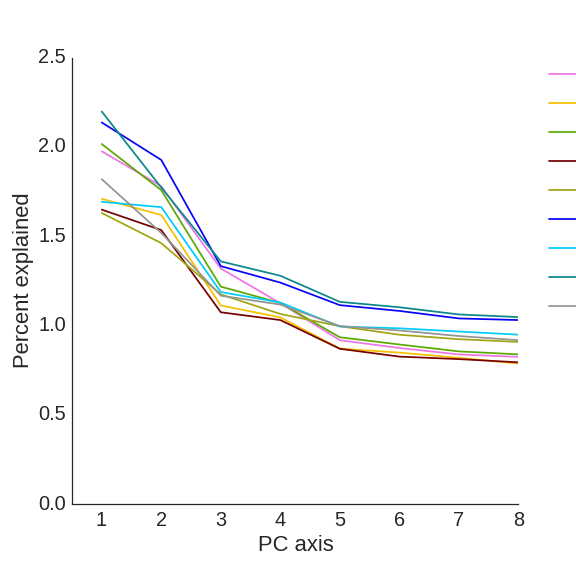
\includegraphics[scale=.4]{figures/supplemental/PCA_eigenvalues.png}
\caption[SUPPLEMENTAL - PCA eigenvalues]{Percent variance explained (eigenvalue) for the first eight PC axes of each locus set.  Notice the similarity between the two bi-allelic sets and the two haplotypic sets.}
\end{figure}

\begin{figure}[H]
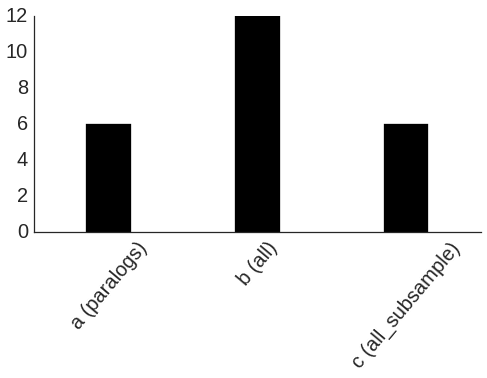
\includegraphics[scale=.4]{figures/supplemental/TW_stats.png}
\caption[SUPPLEMENTAL - PCA significant axes]{Number of significant PC axes as determined by the Tracey-Widom test.}
\end{figure}

\begin{figure}[H]
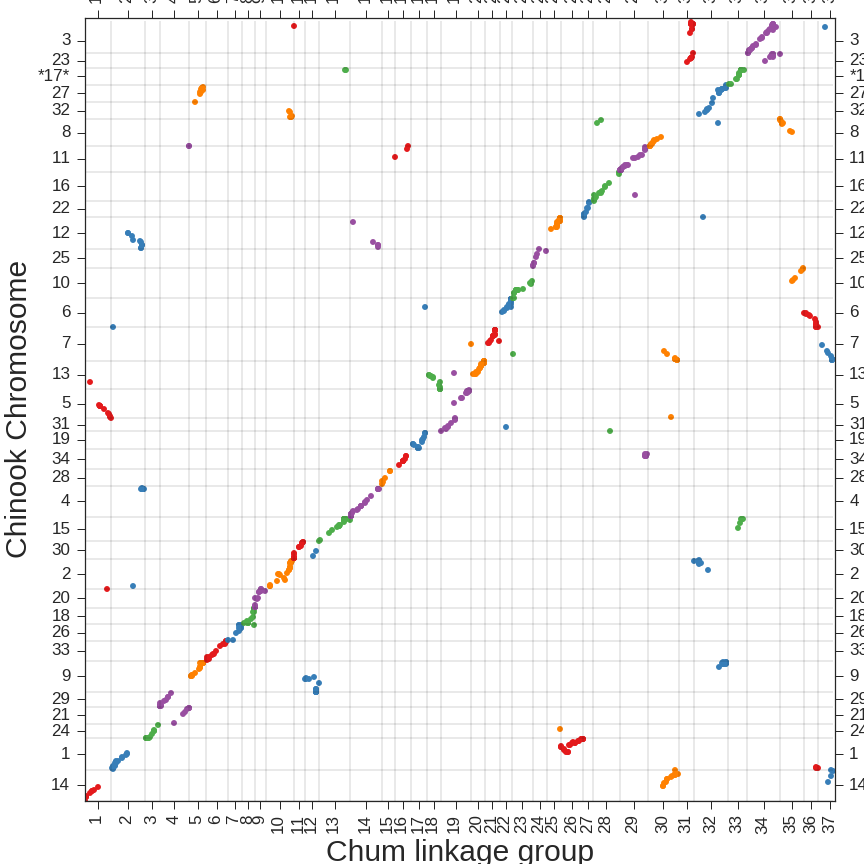
\includegraphics[scale=.35]{figures/supplemental/synteny_chinook.png}
\caption[SUPPLEMENTAL - Chum / Chinook Oxford grid]{Oxford grid - Chum and Chinook linkage groups. Loci are colored by their LG assignment in chum salmon and positioned according to the order within each genome.}
\end{figure}

\bibliographystyle{apalike}
\bibliography{./bibtex/7_13_15}

\section*{Acknowledgements}
WDFW - chum salmon expertise.
Carita Pascal - lab work and library prep.
Samples sources?
Rachel Hovel - multivariate stat advice.
\end{document}